\documentclass[11pt, a4paper]{article}
%\usepackage{proj1}
\usepackage{natbib}
\usepackage{fancyhdr}  
\usepackage{subcaption}
\usepackage{caption}
\usepackage{graphicx}
\usepackage{numprint}
\usepackage{multirow}
\linespread{1.25} 
\setlength{\parindent}{0cm}
\graphicspath{{Images/}}
\usepackage{hyperref}
\usepackage{amsmath}
\usepackage{amsfonts}
\usepackage{amssymb}
\usepackage{amsthm}
\usepackage{mathtools}
\usepackage{commath}
\usepackage{bbm}

%\usepackage[sc,osf]{mathpazo}
\usepackage{subcaption}
\usepackage[a4paper, top=1in, left=1.0in, right=1.0in, bottom=1in, includehead, includefoot]{geometry} %Usually have top as 1in

\usepackage{listings}
\usepackage{color} %red, green, blue, yellow, cyan, magenta, black, white
\definecolor{mygreen}{RGB}{28,172,0} % color values Red, Green, Blue
\definecolor{mylilas}{RGB}{170,55,241}


\hypersetup{colorlinks,linkcolor={black},citecolor={blue},urlcolor={black}}
\usepackage{color}
\urlstyle{same}


\theoremstyle{definition}
\newtheorem{definition}{Definition}[section]

%\newcommand{\Sta}{\rho}
\newcommand{\adja}{q_a}
\newcommand{\adjb}{q_b}
\newcommand{\adjaB}{q_{a,\partial \Omega}}
\newcommand{\adjbB}{q_{b,\partial \Omega}}
%\newcommand{\Con}{u}
\newcommand{\ra}{\rho_a}
\newcommand{\rb}{\rho_b}
\newcommand{\w}{\mathbf{w}}
\newcommand{\Stav}{\mathbf{v}}
\newcommand{\Adja}{\mathbf{p}}
\newcommand{\Adjb}{q}
\newcommand{\Adjc}{{p}_{\partial \Sigma}}
\newcommand{\Con}{\mathbf{f}}
\newcommand{\n}{\mathbf{n}}
\newcommand{\h}{\mathbf{h}}
\newcommand{\K}{\mathbf{K}}


\pagenumbering{gobble}
\begin{document}
	
	
\section{The Multiple Species Gradient Equation}
We consider the derivative of the Lagrangian with respect to $\w$. However, we will need to consider the Frech\'et derivative of terms involving $F(\w)$ first. If $F$ is a function of $\w$ only and not of the position variable $r$, we can do the following. Otherwise, we will have to work with the definition of the Frech\'et derivative and derive the gradient equation like that.
We consider the first order term of the Taylor expansion, so that we have:
\begin{align*}
F(\w + \h) - F(\w) =  \left(\nabla_{\w} F(\w)^T\right) \h 
\end{align*}

Then:
\begin{align*}
\mathcal{L}_{\w}(\ra,\rb, \w, \adja, \adjb) \h  &= \int_0^T \int_\Omega \bigg( \beta \w \cdot \h - D_a \nabla \cdot (\ra \left(\nabla_{\w} F_a(\w)^T\right) \h)  \adja - D_b \nabla \cdot (\rb \left(\nabla_{\w} F_b(\w)^T \right)\h) \adjb \bigg)dr dt \\
&+ \int_0^T \int_{\partial \Omega} \bigg( D_a \ra \left(\nabla_{\w} F_a(\w)^T\right) \h \adjaB   + D_b \rb \left(\nabla_{\w} F_b(\w)^T\right) \h\adjbB     \bigg) \cdot \n dr dt\\
&= \int_0^T \int_\Omega \bigg( \beta \w \cdot \h + D_a \ra \left(\left(\nabla_{\w} F_a(\w)^T\right) \h \right)\cdot\nabla  \adja \\
&+ D_b \rb \left(\left(\nabla_{\w} F_b(\w)^T\right) \h \right)\cdot \nabla \adjb  \bigg)dr dt \\
&- \int_0^T \int_{\partial \Omega} \bigg( D_a \ra \left(\nabla_{\w} F_a(\w)^T\right) \h \adja   + D_b \rb \left(\nabla_{\w} F_b(\w)^T\right) \h\adjb     \bigg) \cdot \n dr dt\\
&+ \int_0^T \int_{\partial \Omega} \bigg( D_a \ra \left(\nabla_{\w} F_a(\w)^T\right) \h \adjaB   + D_b \rb \left(\nabla_{\w} F_b(\w)^T\right) \h\adjbB     \bigg) \cdot \n dr dt\\
&=\int_0^T \int_\Omega \bigg( \beta \w \cdot \h + D_a \ra \left(\left(\nabla_{\w} F_a(\w)^T\right) \h \right)\cdot\nabla  \adja \\
&+ D_b \rb \left(\left(\nabla_{\w} F_b(\w)^T\right) \h \right)\cdot \nabla \adjb  \bigg)dr dt,
\end{align*}
since $\adja = \adjaB$ and $\adjb = \adjbB$ from the adjoint derivation.\\
Now we use the relation $((\nabla \mathbf a)^T)\mathbf b) \cdot \mathbf c= (( \mathbf c \cdot \nabla) \mathbf a ) \cdot \mathbf b$ (from year end review) to find that:
\begin{align*}
\mathcal{L}_{\w}(\ra,\rb, \w, \adja, \adjb) \h  &= \int_0^T \int_\Omega \bigg( \beta \w \cdot \h + D_a \ra \left( \left(\nabla_r \adja \cdot \nabla_{\w} \right) F_a(\w) \right) \cdot \h         \\
&+ D_b \rb \left( \left(\nabla_r \adjb \cdot \nabla_{\w} \right) F_b(\w) \right) \cdot \h       \bigg)dr dt,
\end{align*}
Setting this to zero and since this holds for all permissible $\h$, we get:
\begin{align*}
\beta \w  + D_a \ra \left( \left(\nabla_r \adja \cdot \nabla_{\w} \right) F_a(\w) \right) 
+ D_b \rb \left( \left(\nabla_r \adjb \cdot \nabla_{\w} \right) F_b(\w) \right) = 0.
\end{align*} 
Using that $\nabla \cdot (\mathbf{b a}^T) = \mathbf a (\nabla \cdot \mathbf b) + (\mathbf b \cdot \nabla) \mathbf a$, and observing that $\nabla_{\w} \cdot (\nabla_r q) = 0$, we get:
\begin{align*}
\beta \w  + D_a \ra \nabla_{\w} \cdot \left(\nabla \adja F_a(\w)^T \right) 
+ D_b \rb \nabla_{\w} \cdot \left(\nabla \adjb F_b(\w)^T \right) = 0.
\end{align*} 
Since $\nabla_r q$ does not depend on $\w$ we can rearrange this to get:
\begin{align*}
\beta \w  + D_a \ra \left(\nabla_\w F_a(\w)\right)^T \nabla \adja  
+ D_b \rb \left(\nabla_\w F_b(\w)\right)^T \nabla \adjb = 0.
\end{align*}
And finally we have:
\begin{align*}
\w = - \frac{1}{\beta} \left( D_a \ra \left(\nabla_\w F_a(\w)\right)^T \nabla \adja  
+ D_b \rb \left(\nabla_\w F_b(\w)\right)^T \nabla \adjb \right).
\end{align*}
As an example, take $F_a(\w) = c_a \w$ and $F_b(\w) = c_b \w$. We get:
\begin{align*}
\w  = - \frac{1}{\beta}\bigg( D_a  \ra c_a \mathbf 1 \nabla \adja + D_b \rb c_b \mathbf 1 \nabla \adjb \bigg).
\end{align*}









	
\section{Sedimentation}	

\subsection{Free Energy Frech\'et Derivative}
We have the general expression: 
\begin{align*}
\nabla \cdot \bigg(\rho \nabla \frac{\delta F[\rho]}{\delta \rho}\bigg) &= \frac{1}{\beta} \bigg( \nabla  \cdot \left(  \frac{\nabla \rho}{1 - \eta} \right) - \nabla  \cdot \left(\rho \nabla\frac{\eta - 2}{(\eta - 1)^2} \right) \bigg)\\
&= \frac{1}{\beta} \bigg( \frac{\nabla^2 \rho}{1 - \eta} +  \nabla \rho \cdot \nabla \frac{1}{1 - \eta} - \nabla \rho \cdot \nabla \frac{\eta - 2}{(\eta - 1)^2} - \rho \nabla^2\frac{\eta - 2}{(\eta - 1)^2} \bigg)\\
&= \frac{1}{\beta} \bigg( \frac{\nabla^2 \rho}{1 - \eta} +  \nabla \rho \cdot \nabla \frac{(3- 2 \eta)}{(1 - \eta)^2}  - \rho \nabla^2\frac{\eta - 2}{(\eta - 1)^2} \bigg)
\end{align*}
We want to take the Frech\'et derivative of these terms.
We set:
\begin{align*}
F_1 &= \frac{\nabla^2 \rho}{1 - \eta}= \frac{\nabla^2 \rho}{1 - a \rho}\\
F_2 &= \nabla \rho \cdot \nabla \frac{(3- 2 \eta)}{(1 - \eta)^2} = \nabla \rho \cdot \nabla \frac{(3- 2 a \rho)}{(1 - a \rho)^2} \\
F_3 &= \rho \nabla^2\frac{\eta - 2}{(\eta - 1)^2}= \rho \nabla^2\frac{a \rho - 2}{(a \rho - 1)^2}.
\end{align*}
We are looking at $F(\rho + h) - F(\rho)$. We use the expansions:
\begin{align*}
	\frac{1}{1-x} &= 1 + x + O(x^2)\\
	\frac{1}{(1-x)^2} & = 1 + 2x + O(x^2).
\end{align*}

For $F_1$ we get:
\begin{align*}
F_1(\rho+ h) - F_1(\rho) &= \frac{\nabla^2 (\rho + h)}{1 - a (\rho + h)} - \frac{\nabla^2 \rho}{1 - a \rho}\\
&= \nabla^2 (\rho + h) ( 1 + a(\rho + h)) - \nabla^2 \rho (1 + a \rho)\\
&= (\nabla^2 \rho) ( 1 + a \rho + a h - 1 - a \rho ) + (\nabla^2 h )(1 + a \rho + a h)\\
&= (\nabla^2 \rho) ( a h ) + (\nabla^2 h )(1 + a \rho)\\
\end{align*}
For $F_2$ we have:
\begin{align*}
F_{2}(\rho + h) - F_2(\rho) &= \nabla (\rho + h) \cdot \nabla \frac{(3- 2 a (\rho+h))}{(1 - a (\rho+h))^2} - \nabla \rho \cdot \nabla \frac{(3- 2 a \rho)}{(1 - a \rho)^2}\\
&= \nabla (\rho + h) \cdot \nabla \left( (3- 2 a (\rho+h)) (1 + 2a (\rho+ h))\right) - \nabla \rho \cdot \nabla \left( (3- 2 a \rho) (1 + 2a \rho) \right)\\
&= \nabla (\rho + h) \cdot \nabla \left( 3  + 6a (\rho + h) - 2a (\rho + h) - 4 a^2 (\rho+ h)^2\right) \\
&- \nabla \rho \cdot \nabla \left(3  + 6a \rho - 2a \rho - 4 a^2 \rho^2\right)\\
& = \nabla \rho \cdot \nabla \left(  3  + 4a (\rho + h)  - 4 a^2 (\rho+ h)^2 -  \left(3  + 4a \rho  - 4 a^2 \rho^2\right)           \right)\\
&+ \nabla h \cdot \nabla \left( 3  + 6a (\rho + h) - 2a (\rho + h) - 4 a^2 (\rho+ h)^2\right)\\
& = \nabla \rho \cdot \nabla \left( 4a h  - 8a^2 \rho h \right) + \nabla h \cdot \nabla \left( 3  + 6a \rho  - 2a \rho - 4 a^2\rho^2 \right)\\
&= \nabla \rho \cdot \nabla \left( (4a   - 8a^2 \rho) h \right) + \nabla h \cdot \nabla \left( 4a \rho - 4 a^2\rho^2 \right)\\
&= \nabla \rho \cdot h \nabla \left(4a   - 8a^2 \rho\right) + \nabla \rho \cdot (4a - 8a^2 \rho) \nabla h + \nabla h \cdot \nabla \left( 4a \rho - 4 a^2\rho^2 \right)\\
&= - 8a^2 h \nabla \rho \cdot \nabla \rho  + \nabla h \cdot \left(\nabla \rho (4a - 8a^2 \rho)           + \nabla \left( 4a \rho - 4 a^2\rho^2 \right) \right)\\
&= - 8a^2 h \left(\nabla \rho\right)^2   + \nabla h \cdot \left( 8a \nabla \rho - 16 a^2 \rho \nabla \rho  \right)
\end{align*}
Finally $F_3$ is:
\begin{align*}
F_3(\rho + h) - F_3 (\rho) &= (\rho + h) \nabla^2 \left(\frac{a (\rho + h) - 2}{(a (\rho + h) - 1)^2}\right) - \rho \nabla^2 \left(\frac{a \rho - 2}{(a \rho - 1)^2}\right)\\
&= (\rho + h) \nabla^2 \left( (a (\rho + h) - 2) ( 1 + 2a(\rho +h)) \right) - \rho \nabla^2 \left((a \rho - 2) (1 + 2a \rho) \right)\\
&= (\rho + h) \nabla^2 \left( -2 -3a(\rho + h) + 2a^2 (\rho + h)^2 \right) - \rho \nabla^2 \left(-2 -3a \rho + 2a^2 \rho^2\right)\\
&= \rho \nabla^2 \left( - 3ah + 4a^2 \rho h  \right) + h \nabla^2 \left(-3a \rho  + 2a^2 \rho^2 \right)\\
&= - 3a \rho \nabla ^2 h + 4a^2 \rho \nabla^2(\rho h) - 3ah \nabla^2 \rho + 2a^2 h \nabla^2 \rho^2
\end{align*}


\subsection{Lagrangian}
We consider the part of the Lagrangian that is relevant:
\begin{align*}
\mathcal{L}(\rho, \w, q) = - \int_0^T \int_\Omega \left(\frac{1}{\beta} \bigg( \frac{\nabla^2 \rho}{1 - \eta} +  \nabla \rho \cdot \nabla \frac{(3- 2 \eta)}{(1 - \eta)^2}  - \rho \nabla^2\frac{\eta - 2}{(\eta - 1)^2} \bigg) q \right) dr dt
\end{align*}
Taking the derivatives with respect to $\rho$ gives:
\begin{align*}
\mathcal{L}_\rho(\rho, \w, q) h &= -\frac{1}{\beta}  \int_0^T \int_\Omega \bigg( (\nabla^2 \rho) ( a h ) + (\nabla^2 h )(1 + a \rho) - 8a^2 h \left(\nabla \rho\right)^2   + \nabla h \cdot \left( 8a \nabla \rho - 16 a^2 \rho \nabla \rho  \right) \\
&+ 3a \rho \nabla ^2 h - 4a^2 \rho \nabla^2(\rho h) + 3ah \nabla^2 \rho - 2a^2 h \nabla^2 \rho^2 \bigg) q dr dt
\end{align*}
Integrate by parts the term involving $\nabla^2 (\rho h)$:
\begin{align*}
\int_0^T \int_\Omega q \rho \nabla^2(\rho h) dr dt &= \int_0^T \int_{\partial \Omega} q\rho \nabla(\rho h)\cdot \n dr dt - \int_0^T \int_\Omega \nabla (q \rho) \cdot \nabla (\rho h) dr dt\\
&= \int_0^T \int_{\partial \Omega} q \rho \left(\rho \nabla h + h \nabla \rho \right) \cdot \n dr dt - \int_0^T \int_{\partial \Omega} \rho h \nabla (q\rho) \cdot \n dr dt +
\int_0^T \int_\Omega \rho h \nabla^2 (q\rho)  dr dt\\
&= \int_0^T \int_{\partial \Omega} \left(q \rho^2 \nabla h + q \rho h \nabla \rho  -  \rho^2 h \nabla q - q \rho h \nabla \rho \right)\cdot \n dr dt +
\int_0^T \int_\Omega \rho h \nabla^2 (q\rho)  dr dt\\
&= \int_0^T \int_{\partial \Omega} \left(q \rho^2 \nabla h   -  \rho^2 h \nabla q  \right)\cdot \n dr dt +
\int_0^T \int_\Omega \rho h \nabla^2 (q\rho)  dr dt\\
\end{align*}
Then we have the terms involving $\nabla^2 h$:
\begin{align*}
\int_0^T \int_\Omega  (\nabla^2 h) (q + 4 a q \rho )  dr dt &= \int_0^T \int_{\partial \Omega}(\nabla h) (q + 4 a q \rho ) \cdot \n dr dt - \int_0^T \int_\Omega (\nabla h) \cdot \nabla (q + 4 a q \rho )dr dt\\
&= \int_0^T \int_{\partial \Omega} \left((\nabla h) (q + 4 a q \rho ) -  h \nabla q -4 ah \nabla (q \rho ) \right) \cdot \n  dr dt \\
&+ \int_0^T \int_\Omega  h\nabla^2 q + 4 a h \nabla^2(q \rho ) dr dt\\
&= \int_0^T \int_{\partial \Omega} \left((\nabla h) (q + 4 a q \rho ) -  h \nabla q - 4 ah \nabla (q \rho ) \right) \cdot \n  dr dt \\
&+ \int_0^T \int_\Omega  h\nabla^2 q + 4 a h q \nabla^2 \rho + 4 a h  \rho \nabla^2 q + 4 a h \nabla \rho \cdot \nabla q dr dt
\end{align*}
Finally, the terms involving $\nabla h$:
\begin{align*}
\int_0^T \int_\Omega \nabla h \cdot \left( 8a q\nabla \rho - 16 a^2 q \rho \nabla \rho  \right) dr dt &= \int_0^T \int_{\partial \Omega}  h \left( 8a q \nabla \rho - 16 a^2 q\rho \nabla \rho  \right) \cdot \n dr dt \\
&- \int_0^T \int_\Omega h \nabla \cdot\left( 8a q \nabla \rho - 16 a^2 q\rho \nabla \rho  \right) dr dt\\
& = \int_0^T \int_{\partial \Omega}  h \left( 8a q\nabla \rho - 16 a^2 q \rho \nabla \rho  \right) \cdot \n dr dt \\
&- \int_0^T \int_\Omega h \left( 8a \nabla \cdot( q \nabla \rho) - 16 a^2 \nabla \cdot (q\rho \nabla \rho ) \right) dr dt\\
& = \int_0^T \int_{\partial \Omega}  h \left( 8a q\nabla \rho - 16 a^2 q \rho \nabla \rho  \right) \cdot \n dr dt \\
&- \int_0^T \int_\Omega h \bigg( 8a \nabla q \cdot \nabla \rho + 8aq \nabla^2 \rho  \\
&- 16 a^2 q (\nabla \rho)^2 - 16 a^2 \rho \nabla \rho \cdot \nabla q - 16 a^2 q \rho \nabla^2 \rho \bigg) dr dt\\
\end{align*}
Combining all of these gives:
\begin{align*}
\mathcal{L}_\rho(\rho, \w, q) h &= -\frac{1}{\beta}  \int_0^T \int_\Omega \bigg(q (\nabla^2 \rho) ( a h )  -q 8a^2 h \left(\nabla \rho\right)^2   \\
&+  8a h\nabla q \cdot \nabla \rho + 8aq h\nabla^2 \rho - 16 a^2 q h(\nabla \rho)^2 - 16h a^2 \rho \nabla \rho \cdot \nabla q - 16 ha^2 q \rho \nabla^2 \rho \\
& - 4a^2 \rho h q\nabla^2(\rho ) - 8a^2 \rho h \nabla q \cdot \nabla \rho  - 4a^2 h \rho^2 \nabla^2 q  + 3ah q\nabla^2 \rho - 2a^2qh \nabla^2 \rho^2\\
&h\nabla^2 q + 4 a h q \nabla^2 \rho + 4 a h  \rho \nabla^2 q + 4 a h \nabla \rho \cdot \nabla q \bigg)  dr dt
\end{align*}
Rearranging and cancelling results in:

\begin{align*}
\mathcal{L}_\rho(\rho, \w, q) h &= -\frac{1}{\beta}  \int_0^T \int_\Omega h q \bigg( a\nabla^2 \rho -8a^2  \left(\nabla \rho\right)^2 + 8a\nabla^2 \rho - 16 a^2 (\nabla \rho)^2 \\
&- 16 a^2  \rho \nabla^2 \rho - 4a^2 \rho \nabla^2(\rho ) +3a\nabla^2 \rho - 2a^2 \nabla^2 \rho^2 + 4 a \nabla^2 \rho
 \bigg)\\
&+ h \nabla q \cdot \bigg( 8a \nabla \rho - 16 a^2 \rho \nabla \rho- 8a^2 \rho  \nabla \rho + 4 a  \nabla \rho \bigg)\\
&+ h \nabla^2 q \bigg( 1  - 4a^2  \rho^2  + 4 a   \rho  \bigg) dr dt
\end{align*}



\begin{align*}
\mathcal{L}_\rho(\rho, \w, q) h &= -\frac{1}{\beta}  \int_0^T \int_\Omega h q \bigg(16 a\nabla^2 \rho -28a^2  \left(\nabla \rho\right)^2   - 24 a^2  \rho \nabla^2 \rho  
\bigg)\\
&+ h \nabla q \cdot \bigg( 12a \nabla \rho - 24 a^2 \rho \nabla \rho  \bigg) + h \nabla^2 q \bigg( 1  - 4a^2  \rho^2  + 4 a   \rho  \bigg) dr dt
\end{align*}


Adding the other terms to it we get the adjoint equation:
\begin{align*}
\frac{\partial q}{\partial t} =& -\frac{1}{\beta} q \bigg(16 a\nabla^2 \rho -28a^2  \left(\nabla \rho\right)^2   - 24 a^2  \rho \nabla^2 \rho  
\bigg)\\
&-\frac{1}{\beta} \nabla q \cdot \bigg( 12a \nabla \rho - 24 a^2 \rho \nabla \rho  \bigg) -\frac{1}{\beta}  \nabla^2 q \bigg( 1  - 4a^2  \rho^2  + 4 a   \rho  \bigg) \\
& + \nabla V_{ext} \cdot \nabla q - \w \cdot \nabla q - \rho + \widehat \rho + \int_\Omega ( \nabla_r q(r) - \nabla_{r'} q(r')) \rho(r') \K(r,r') dr'
\end{align*}


\subsection{Boundary Terms}
We had the flux term:
\begin{align*}
-\rho \nabla \frac{\delta F[\rho]}{\delta \rho} &= -\frac{1}{\beta} \bigg( \nabla \rho +   \frac{\rho \nabla \eta}{1 - \eta} - \rho \nabla\frac{\eta - 2}{(\eta - 1)^2}  \bigg)\\
&=- \frac{1}{\beta} \bigg( \nabla \rho +   \frac{\eta\nabla \rho}{1 - \eta} - \rho \nabla\frac{\eta - 2}{(\eta - 1)^2}  \bigg)\\
&= -\frac{1}{\beta} \bigg( \nabla \rho + \frac{\nabla \rho}{1 - \eta} - \nabla \rho - \rho \nabla\frac{\eta - 2}{(\eta - 1)^2}  \bigg)\\
&= -\frac{1}{\beta} \bigg(  \frac{\nabla \rho}{1 - \eta}  - \rho \nabla\frac{\eta - 2}{(\eta - 1)^2}  \bigg)
\end{align*}

Taking Frech\'et derivatives gives:
\begin{align*}
F_4(\rho+h) - F(\rho) &= \nabla(\rho+h) (1 + a\rho + ah) - \nabla \rho (1 + a \rho)\\
&=(\nabla \rho)(ah) + \nabla h (1 + a \rho)\\
&= ah \nabla \rho + \nabla h + a \rho \nabla h, 
\end{align*}
and
\begin{align*}
F_5(\rho+ h)- F_5(\rho) &= (\rho + h) \nabla \left((a \rho + a h - 2) ( 1 + 2a \rho + 2 a h)\right) - \rho \nabla \left((a \rho - 2)(1 + 2a \rho)\right)\\&= 
\rho \nabla (a \rho + 2a^2 \rho + 2 a^2 \rho h + ah + 2a^2\rho h + 2 a^2 h^2 -2 -4a \rho - 4ah)\\
&- \rho \nabla( a\rho + 2a^2 \rho^2 -2 -4a\rho)\\
&+h \nabla (a \rho + 2a^2 \rho + 2 a^2 \rho h + ah + 2a^2\rho h + 2 a^2 h^2 -2 -4a \rho - 4ah)\\
&= \rho \nabla \left(4a^2 \rho h -3ah \right)\\
&+h \nabla \left( 2a^2 \rho -2 -3a \rho\right)\\
&= 4a^2 \rho^2 \nabla h + 4a^2 h \rho \nabla \rho - 3a \rho \nabla h + 2a^2 h \nabla \rho - 3a h \nabla \rho
\end{align*}

Then the contribution to the Lagrangian is:
\begin{align*}
\mathcal{L}(\rho, \w, q) = \int_0^T \int_{\partial \Omega} -\frac{1}{\beta} \bigg(  \frac{\nabla \rho}{1 - \eta}  - \rho \nabla\frac{\eta - 2}{(\eta - 1)^2}  \bigg)\cdot \n dr dt.
\end{align*}
Then the contribution to the derivative with respect to $\rho$ is:
\begin{align*}
\mathcal{L}_{\rho,1} (\rho, \w, q)h &= \frac{1}{\beta} \int_0^T \int_{\partial \Omega} \bigg(ah \nabla \rho + \nabla h + a \rho \nabla h \\
& -4a^2 \rho^2 \nabla h - 4a^2 h \rho \nabla \rho + 3a \rho \nabla h - 2a^2 h \nabla \rho + 3a h \nabla \rho \bigg) q_{\partial \Omega} \cdot \n  dr dt\\
&= \frac{1}{\beta} \int_0^T \int_{\partial \Omega} \bigg( \nabla h( 1 + a\rho - 4a^2 \rho^2 + 3a \rho) +h(4a \nabla \rho -4a^2 \rho \nabla \rho -2a^2 \nabla \rho )\bigg) q_{\partial \Omega} \cdot \n dr dt
\end{align*}
Now, collecting the boundary terms from integrating by parts in the main body we get:
\begin{align*}
\mathcal{L}_{\rho,2} (\rho, \w, q)h&=- \frac{1}{\beta}\int_0^T \int_{\partial \Omega} \bigg((-4a^2 q\rho^2 \nabla h - \rho^2 h \nabla q )\\
&+(\nabla h (q+ 4aq\rho) -h \nabla q - 4ah \nabla (q \rho))\\
&+h(8aq \nabla \rho - 16a^2 q \rho \nabla \rho) \bigg) \cdot \n dr \\
&= - \frac{1}{\beta}\int_0^T \int_{\partial \Omega} \bigg(\nabla h (- 4a^2 q \rho^2 +q + 4aq\rho)\\
&+ h(- \rho^2 \nabla q - \nabla q -4a\rho\nabla q  + 4a q\nabla \rho - 16a^2 q \rho \nabla \rho) \bigg) \cdot \n dr dt
\end{align*}
Combining the two gives:
\begin{align*}
\mathcal{L}_{\rho} (\rho, \w, q)h &= \frac{1}{\beta} \int_0^T \int_{\partial \Omega} \nabla h \bigg(  q_{\partial \Omega} + aq_{\partial \Omega}\rho - 4a^2q_{\partial \Omega} \rho^2 + 3a q_{\partial \Omega}\rho + 4a^2 q \rho^2 -q - 4aq\rho \bigg) \cdot \n\\
&+ h \bigg(  4a q_{\partial \Omega}\nabla \rho -4a^2 q_{\partial \Omega}\rho \nabla \rho -2a^2q_{\partial \Omega} \nabla \rho             
+\rho^2 \nabla q + \nabla q +4a\rho\nabla q  - 4a q\nabla \rho + 16a^2 q \rho \nabla \rho\bigg) \cdot \n dr dt
\end{align*}

Considering $h =0$ and $\nabla h \neq 0$ on $\partial \Omega$ we get that:
\begin{align*}
\bigg(  q_{\partial \Omega} + aq_{\partial \Omega}\rho - 4a^2q_{\partial \Omega} \rho^2 + 3a q_{\partial \Omega}\rho + 4a^2 q \rho^2 -q - 4aq\rho \bigg) \cdot \n = 0
\end{align*}
Equating this for powers of $\rho$ (allowed?) we conclude that $q_{\partial \Omega} = q$. Then if $h \neq 0$ we get:
\begin{align*}
\bigg( -2a^2q \nabla \rho             
+\rho^2 \nabla q + \nabla q +4a\rho\nabla q   + 12a^2 q \rho \nabla \rho\bigg) \cdot \n =0
\end{align*}
Since this doesn't cancel, there may be a mistake in the calculations.

\subsection{Implementation}
While there is probably a mistake in the above, I implemented this as flow control problem. I set the target to be the forward problem with a certain $V_{ext}$ and the initial configuration has a bit of a weaker $V_{ext}$, so that we would need some more help from the flow term to get to the first one. However, the difference is $a0 = 0.1$, $a1 =0.099$, so that it's hard to see what the difference actually is, see Figures \ref{F01}, \ref{F02} and \ref{F03}. It may be better to actually do $V_{ext}$ control?
\begin{figure}[h]
	\centering
	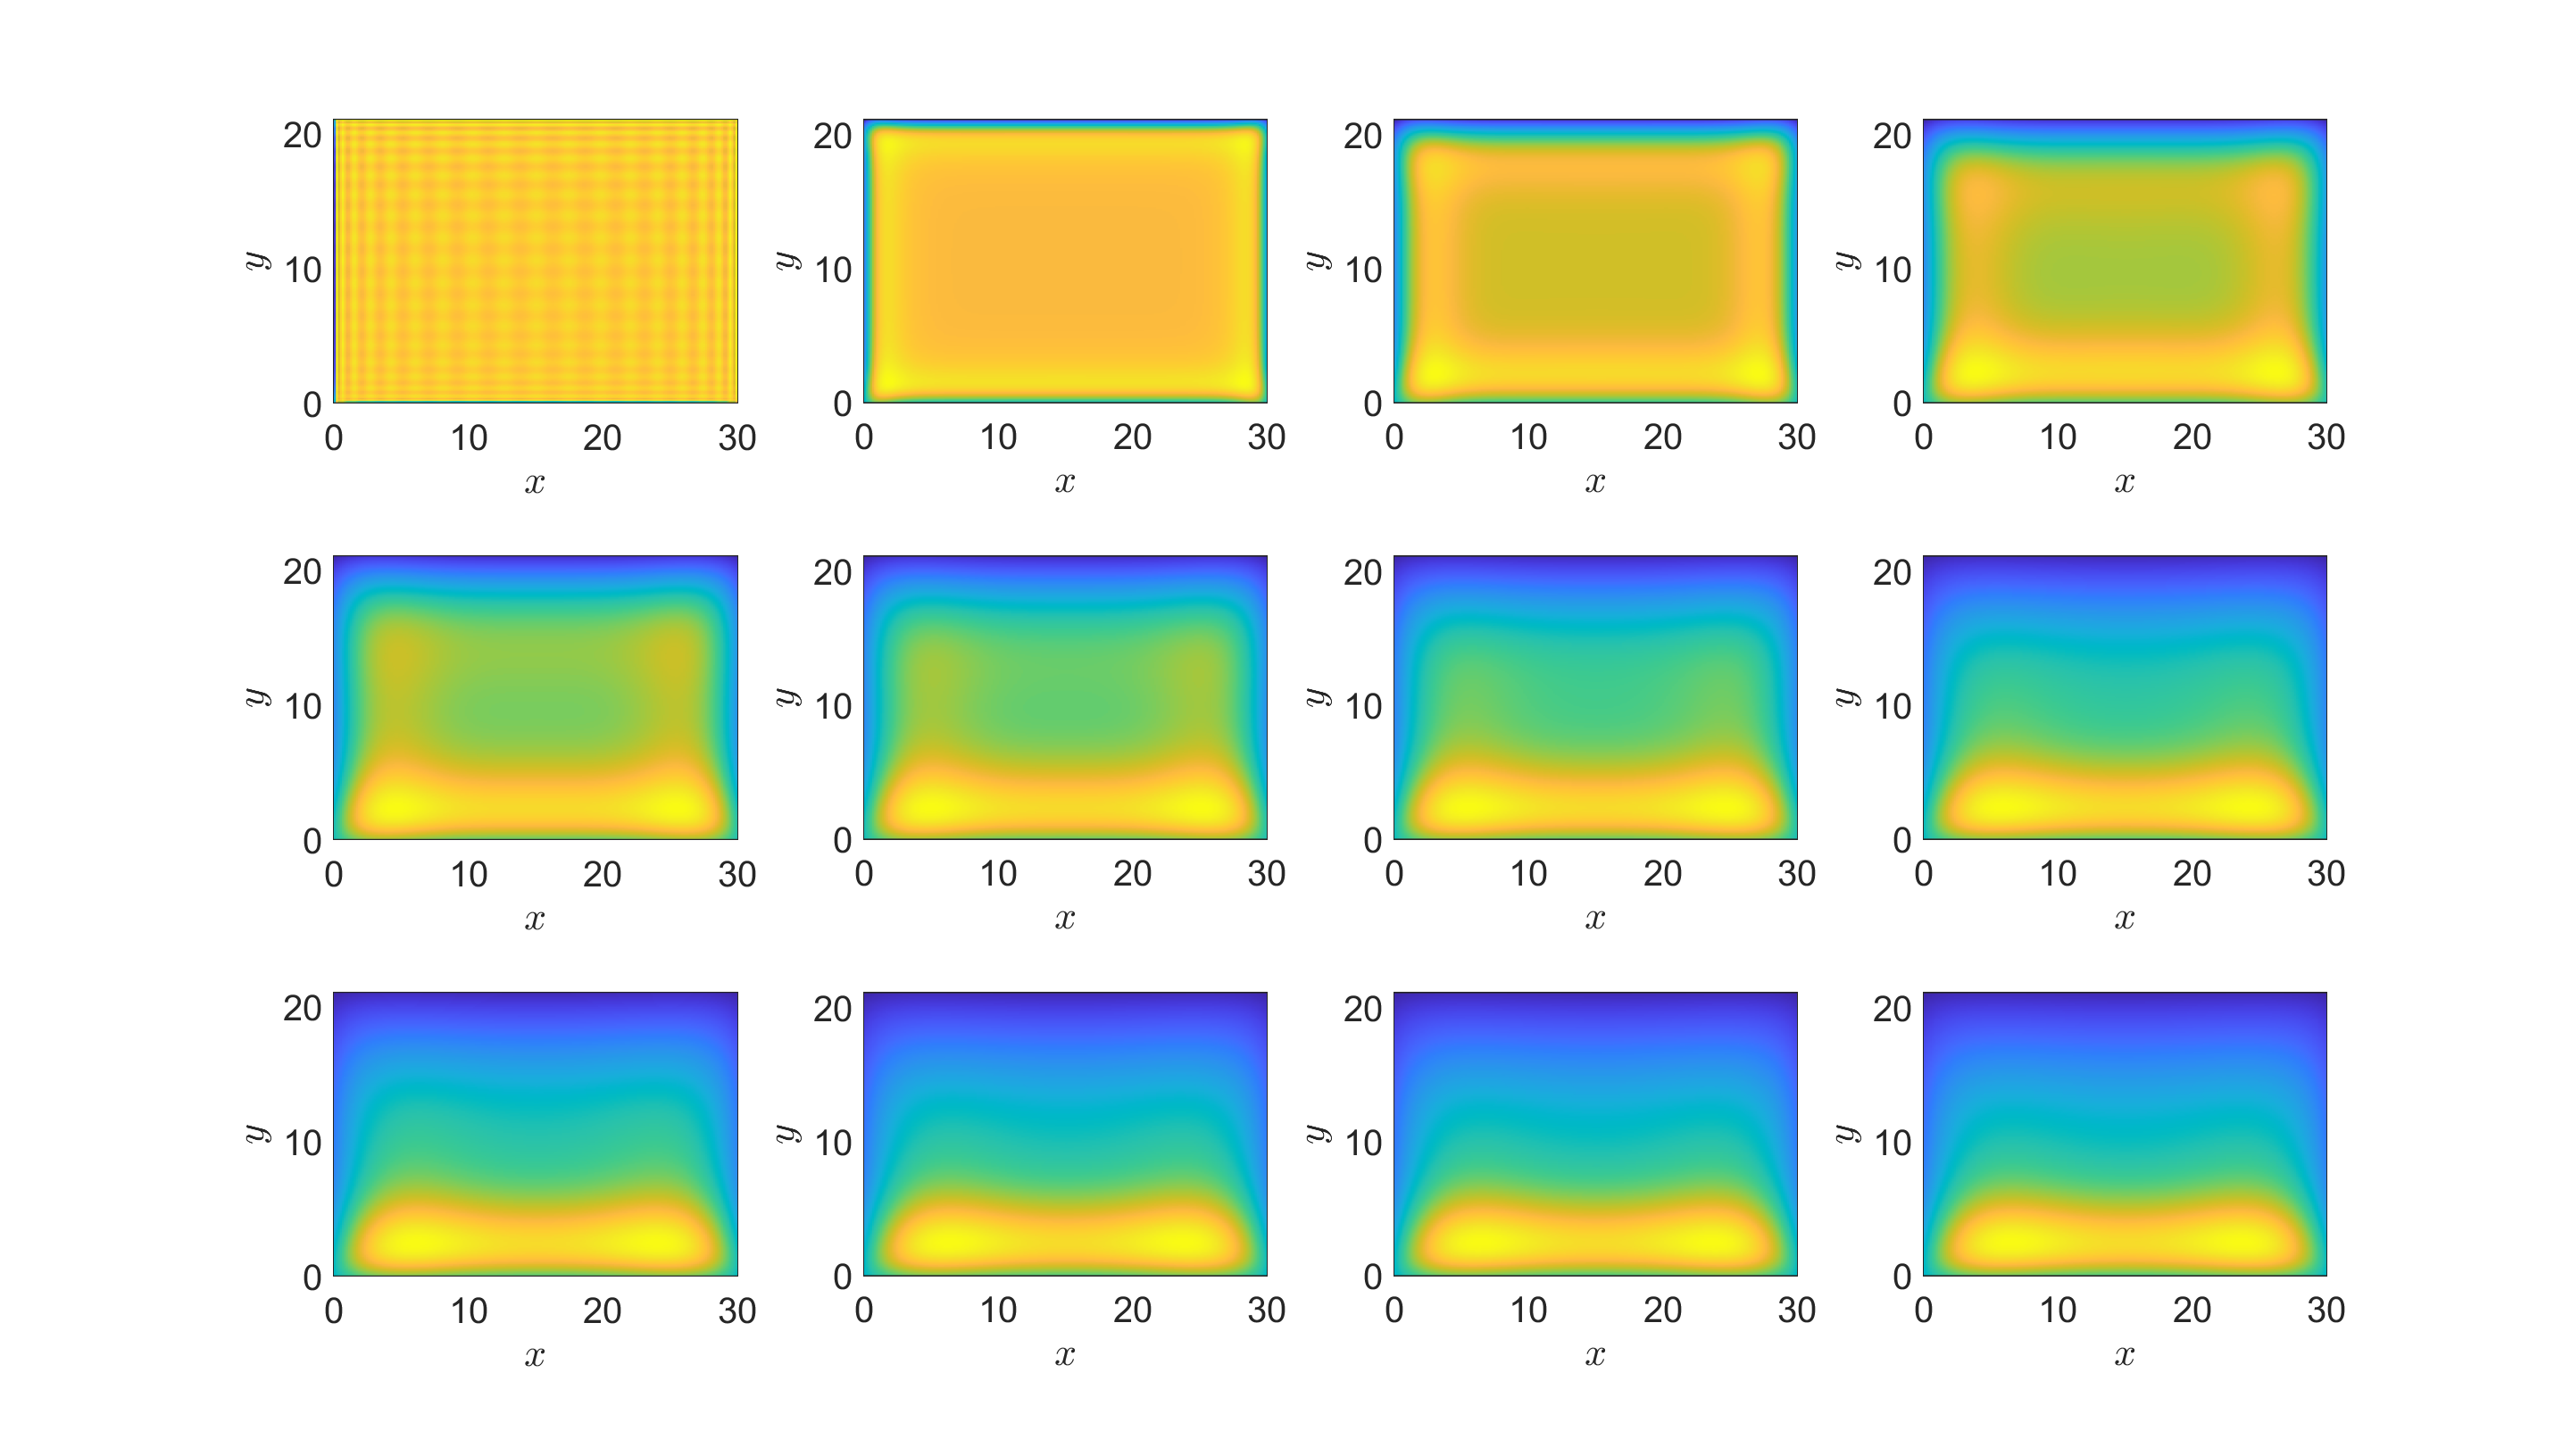
\includegraphics[scale=0.2]{FW1.png}
	\caption{Sedimentation Forward Problem, $a = 0.099$} 
	\label{F01}
\end{figure} 

\begin{figure}[h]
	\centering
	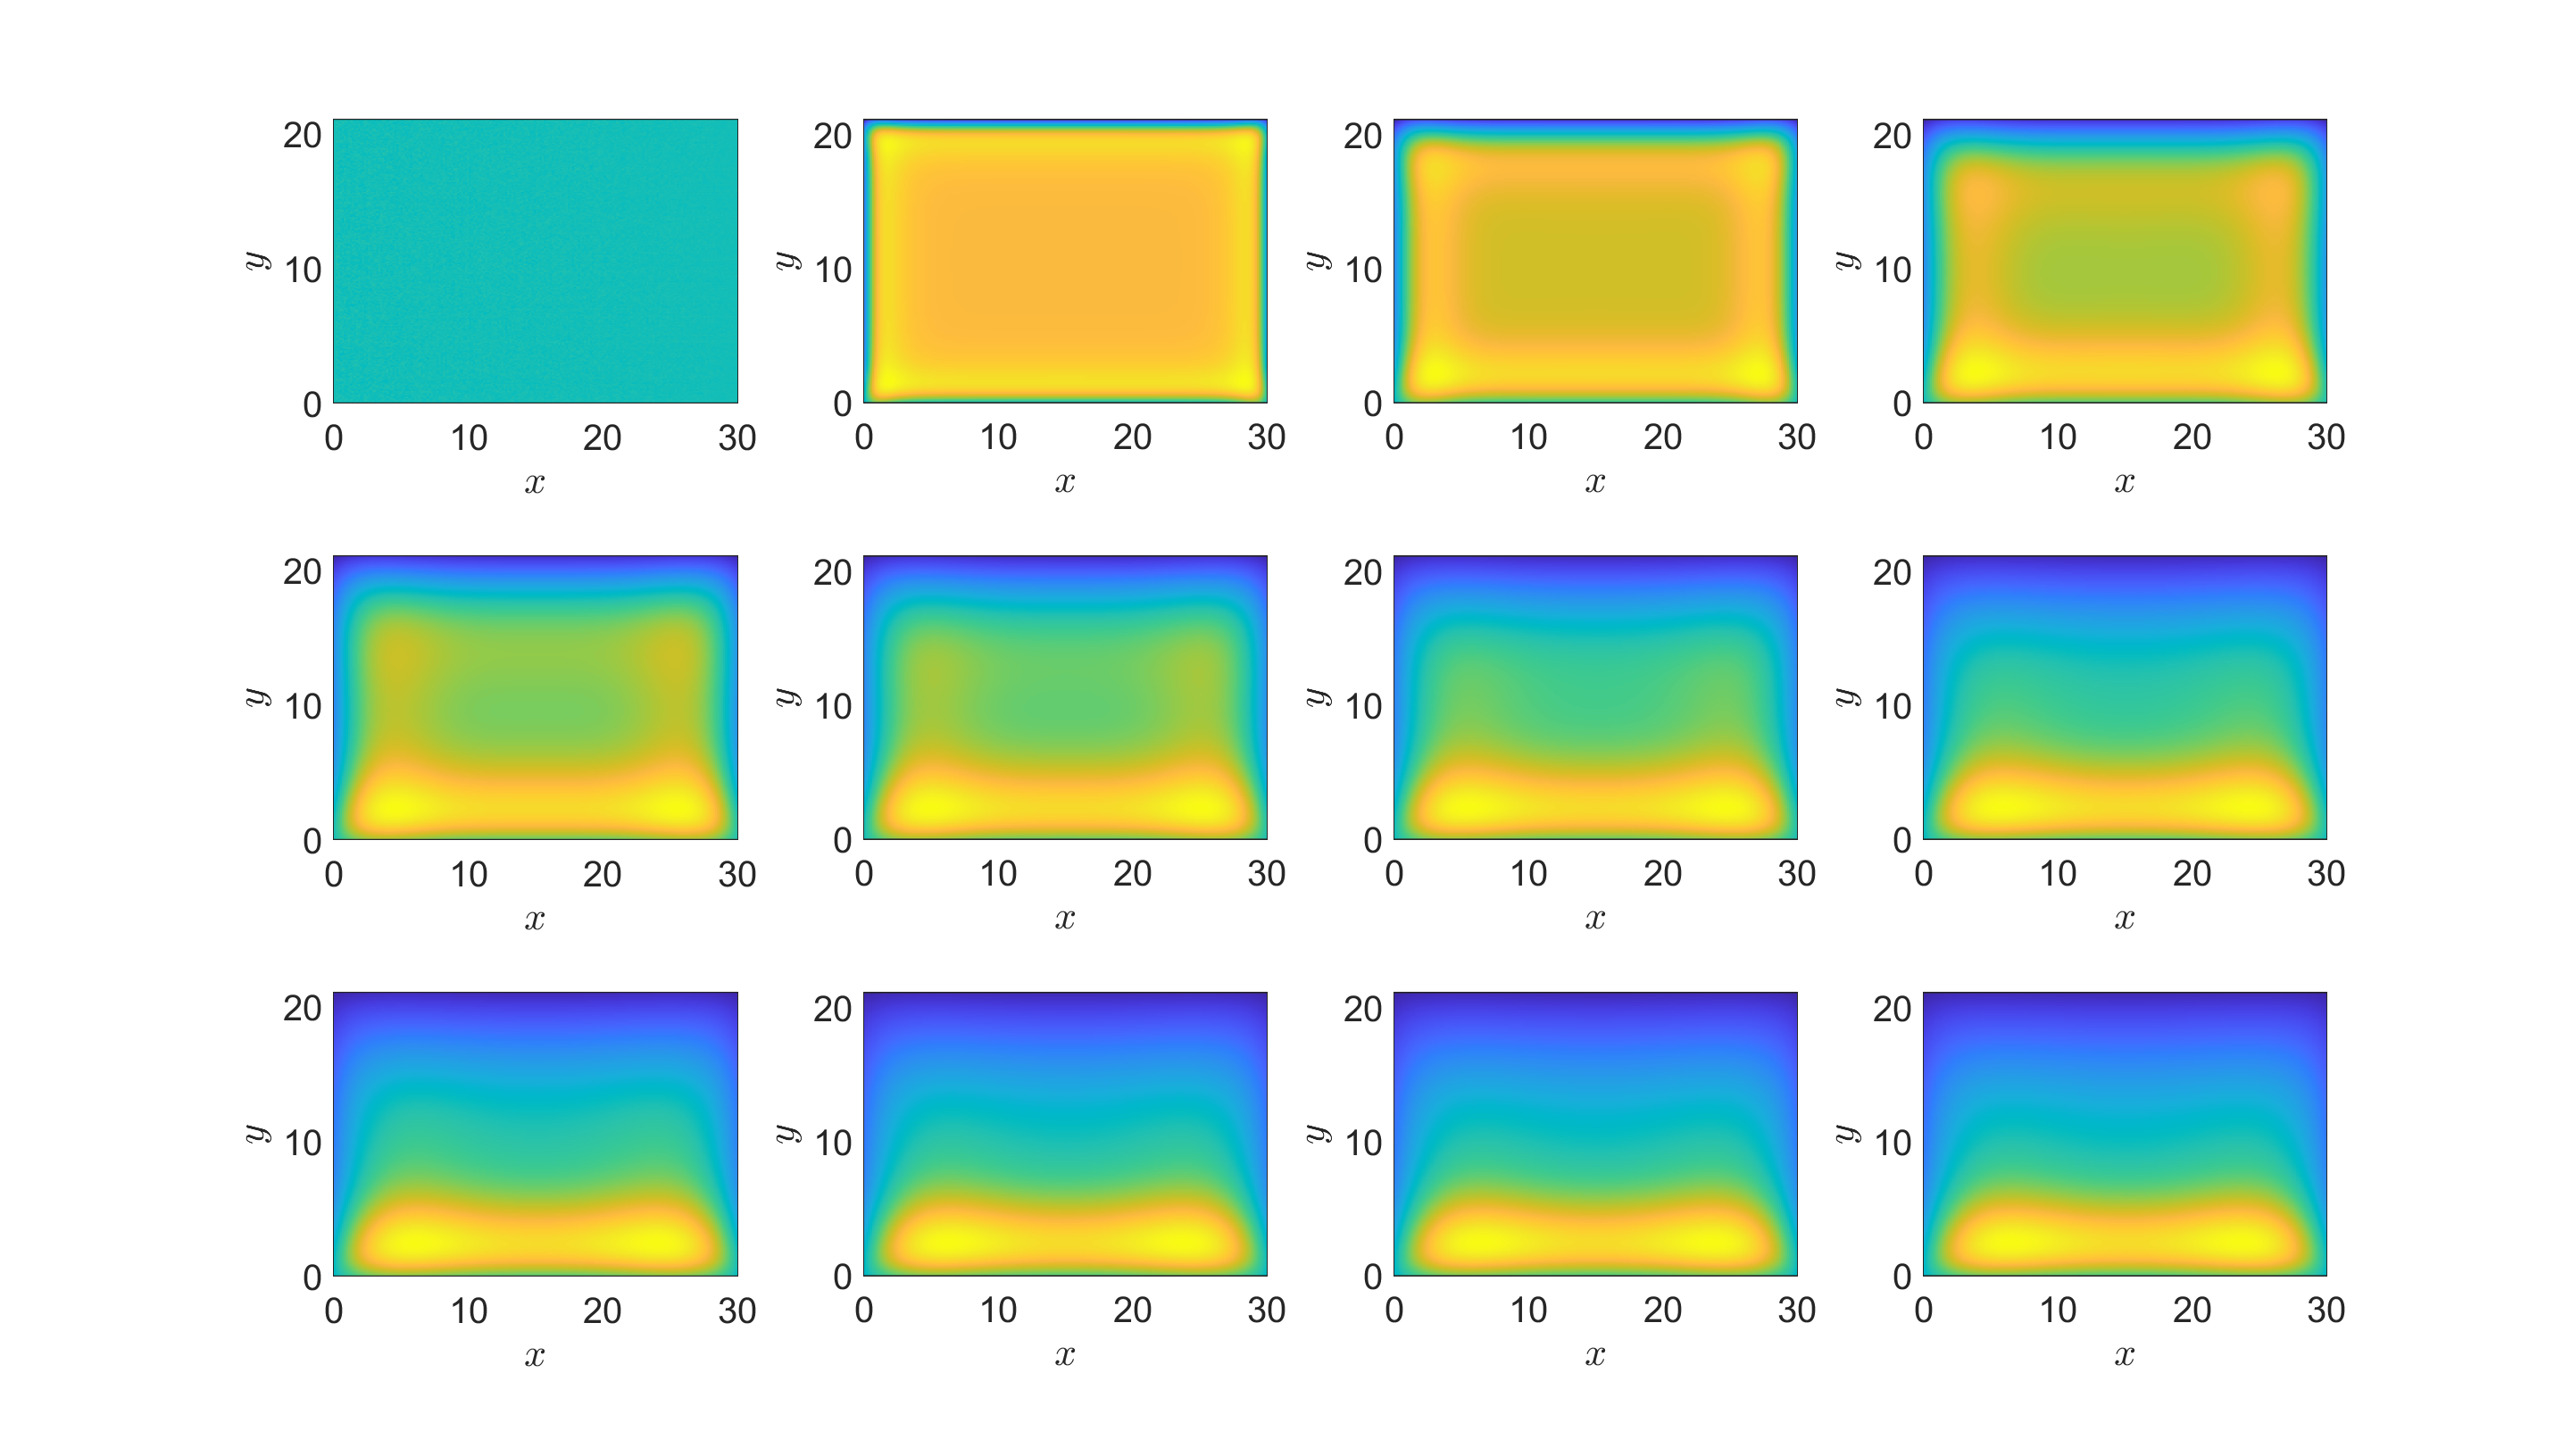
\includegraphics[scale=0.2]{Opt1.png}
	\caption{Sedimentation Optimal $\rho$, target $a =0.1$} 
	\label{F03}
\end{figure} 
\begin{figure}[h]
	\centering
	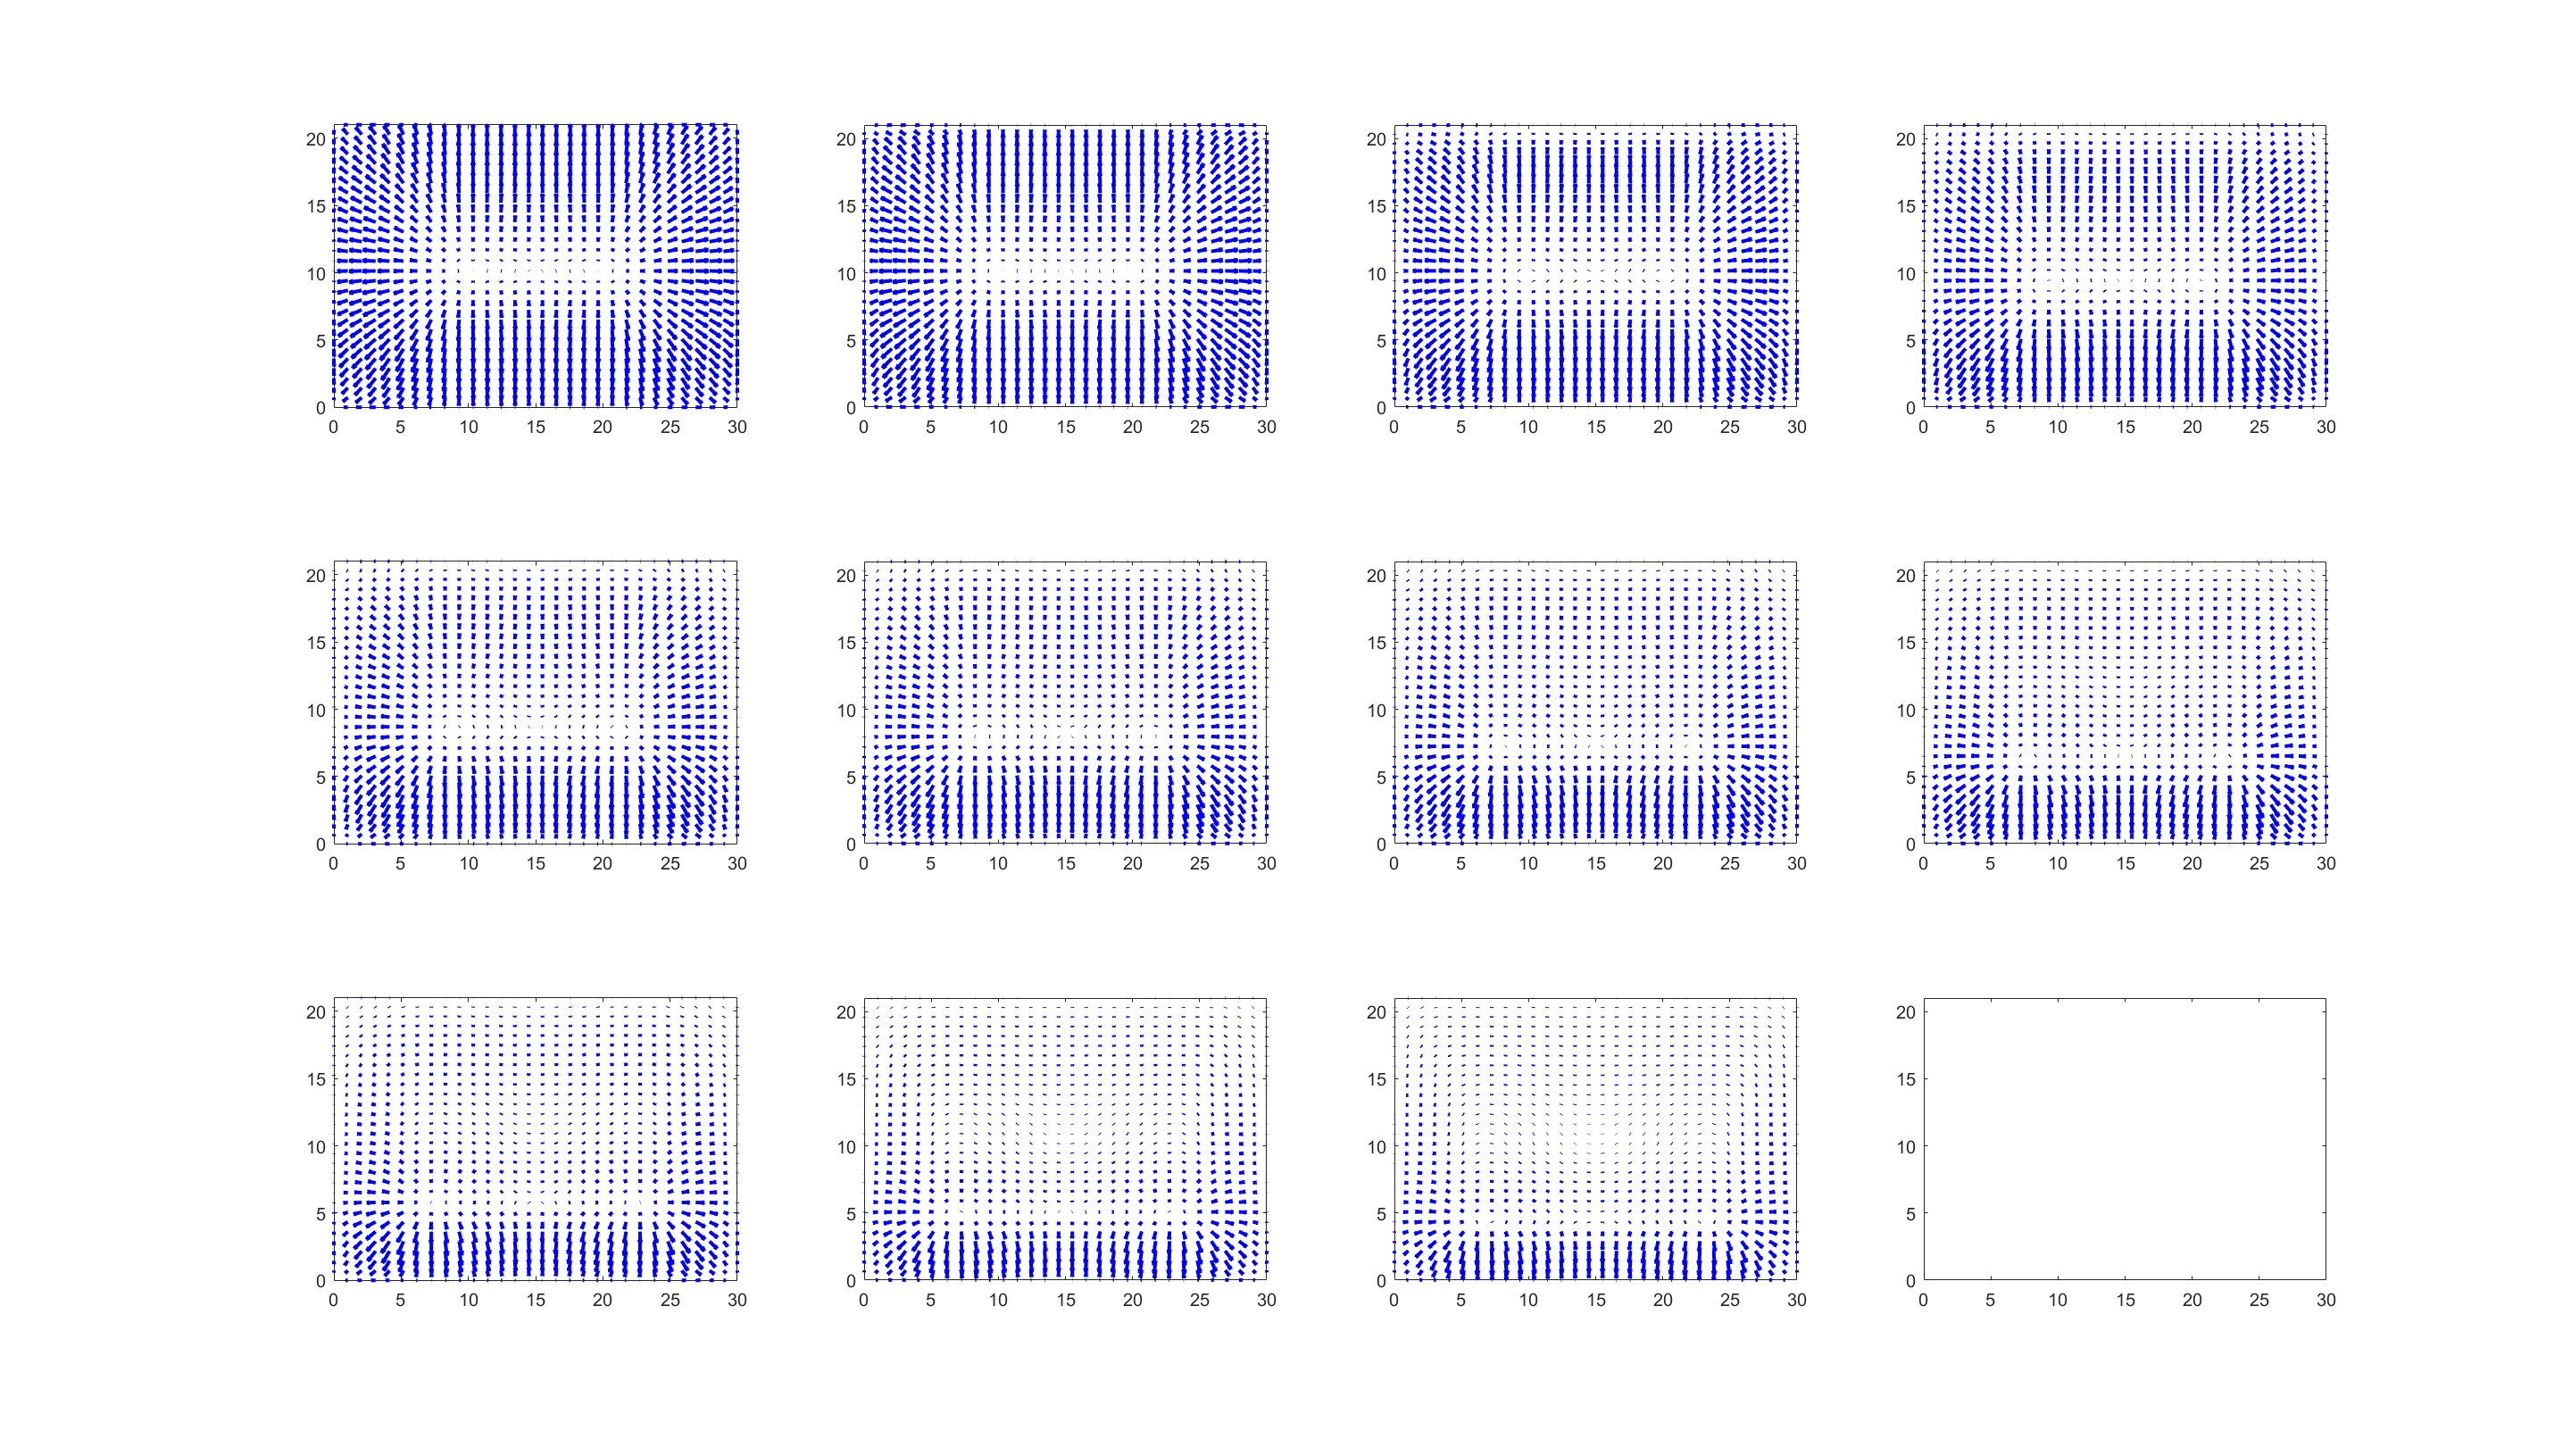
\includegraphics[scale=0.2]{C1.png}
	\caption{Sedimentation Control} 
	\label{F02}
\end{figure} 

\section{Constriction Example Equation}
We have the equation
\begin{align*}
\frac{\partial \rho}{\partial t} = \nabla^2 \rho + \nabla( \rho \nabla V_{ext}).
\end{align*}
We then make the substitution $\rho = e^{h - V_{ext}}$.
Then 
\begin{align*}
\frac{\partial \rho}{\partial t} &= \frac{\partial}{\partial t} e^{h - V_{ext}} = e^{h - V_{ext}}\frac{\partial h}{\partial t}\\
\nabla \rho &= \nabla e^{h - V_{ext}} = e^{h - V_{ext}} \nabla(h - V_{ext})\\
\nabla^2 \rho &= \nabla \bigg(e^{h - V_{ext}}\nabla(h - V_{ext}) \bigg) \\
&= e^{h - V_{ext}} \bigg(\nabla^2 h - \nabla^2 V_{ext} \bigg) + e^{h - V_{ext}} \bigg( (\nabla h)^2 - 2 \nabla h \cdot \nabla V_{ext} + (\nabla V_{ext})^2 \bigg)\\
\nabla\bigg(\rho \nabla V_{ext}\bigg) &= \nabla( e^{h - V_{ext}} \nabla V_{ext}) = e^{h - V_{ext}} \nabla^2 V_{ext} + e^{h - V_{ext}} \bigg(\nabla h \cdot \nabla V_{ext} - (\nabla V_{ext})^2  \bigg)
\end{align*}
Then we get:
\begin{align*}
\frac{\partial h}{\partial t} &= \nabla^2 h - \nabla^2 V_{ext} + (\nabla h)^2 - 2 \nabla h \cdot \nabla V_{ext} + (\nabla V_{ext})^2 +\nabla^2 V_{ext} + \nabla h \cdot \nabla V_{ext} - (\nabla V_{ext})^2\\
&= \nabla^2 h + (\nabla h)^2 - \nabla h \cdot \nabla V_{ext} 
\end{align*}

Problem: This crashes in the implementation, so either it's the wrong equation or the implementation is wrong.

\section{Periodic Box}
I am not sure yet what this is doing (the scaling of the box and the periodicity). Gravity is acting from left to right, top and bottom are periodic. Can we change that? See Figure \ref{F1}.
\begin{figure}[h]
	\centering
	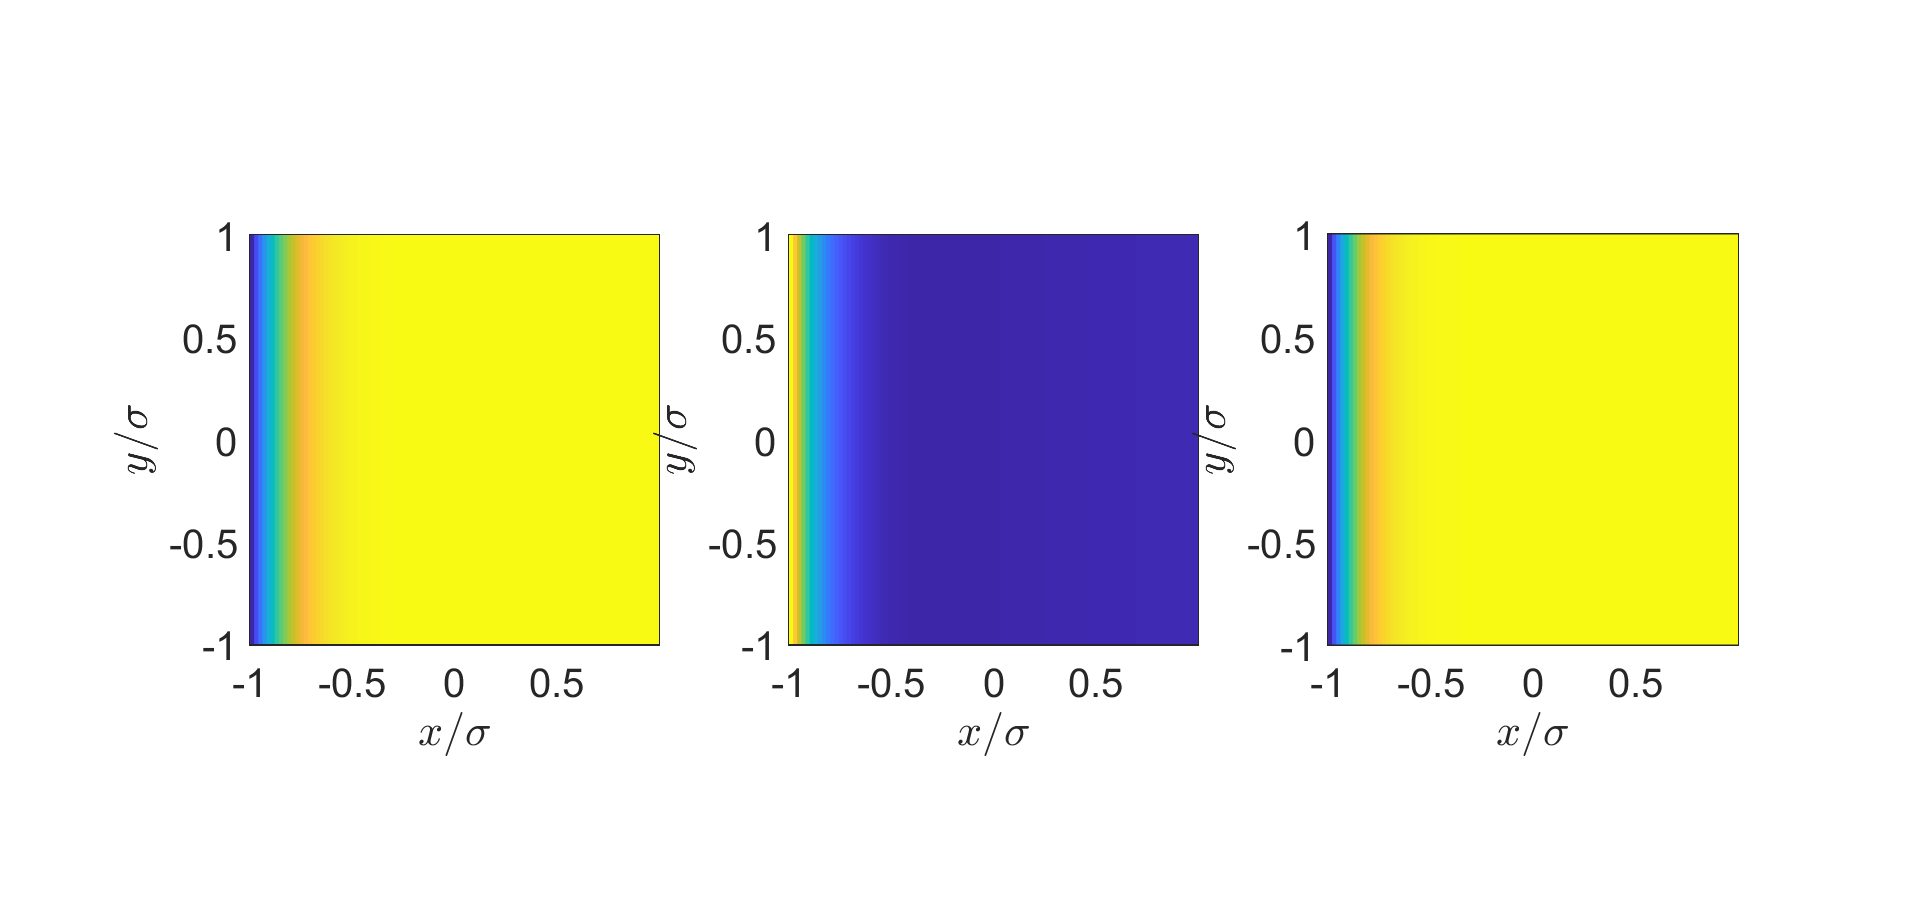
\includegraphics[scale=0.25]{P1.png}
	\caption{Periodic Box 1} 
	\label{F1}
\end{figure} 

\section{CV}
Questions:\\
Cover letter: How much detail of what I am doing/ how technical? What else should I include about myself?\\
CV: Should I include the preprint? Is the order of sections correct? What level of Matlab skills do I have?
\end{document}

